\section{面向高亏格的 GW 理论导引 (Patrick Lei)}%
\label{sec:Intro to GW theory with a view to higher genus (Patrick Lei)}


\subsection{GW 理论导引}%
\label{sub:Introduction to GW theory}

关于虚基本类的构造，见~\cite{BehrendFantechi1997}；关于公理与量子上同调，见~\cite{KM1994}。

这些讲座的目标是以一种便于在高亏格中进行计算的方式来讨论 Gromov-Witten 理论。Gromov-Witten 理论研究模空间 \(\Mbar_{g,n}(X, \beta)\) 上的积分，其中 \(X\) 是光滑射影代数簇，\(\beta \in H_2(X, \Z)\) 是有效曲线类。有图表
\begin{equation*}
\begin{tikzcd}
    \mc{C} \ar{r}{f} \ar[bend right=20]{d}[swap]{\pi} & X \\
    \Mbar_{g,n}(X, \beta) \ar[bend right=20]{u}[swap]{\sigma_i} \ar{ur}[swap]{\on{ev}_i}
\end{tikzcd}
\end{equation*}
其中 \(\mc{C}\) 是万有曲线，\(\sigma_i\) 是 \(\pi\) 的给出标记点的截面，\(f\) 是万有稳定映射，而 \(\ev_i = f \circ \sigma_i\) 是求值态射。虽然 \(\Mbar_{g,n}(X, \beta)\) 一般是奇异的、非等维的且可约的，但存在一个特殊类
\[ [\Mbar_{g,n}(X, \beta)]^{\vir} \in A_{\ab(c_1(X), \beta) + (\dim X - 3)(1-g) + n}(\Mbar_{g,n}(X, \beta), \Q), \]
称为 \textit{虚基本类}。

\begin{exer}
    用形变理论中的标准论证验证 \(\Mbar_{g,n}(X, \beta)\) 的“预期维数”就是上面给出的数。
\end{exer}

在 \(X\) 光滑且射影的假设下，\(\Mbar_{g,n}(X, \beta)\) 是真的，因此我们可以定义 \textit{GW 不变量}
\[ \ab<\tau_{a_1}(\alpha_1), \cdots, \tau_{a_n}(\alpha_n)>_{g,n,\beta} \coloneqq \int_{[\Mbar_{g,n}(X, \beta)]^{\vir}} \prod_{i=1}^n \ev_i^* \alpha_i \cdot \psi_i^{a_i} \]
对 \(\alpha_i \in H^*(X)\)。这里，\(\psi_i\) 由 \(\psi_i = c_1(\sigma_i^*(\omega_{\pi}))\) 定义。

遗憾的是，计算单个 Gromov-Witten 不变量非常困难，因此我们将考虑一个更困难的问题：研究 GW 不变量的生成级数，例如
\[ F_g = \sum_{\beta \geq 0} q^{\beta} \ab<>_{g,0,\beta} \]
其中 \(X\) 是 Calabi-Yau 三维簇。这里，\(q\) 是记录曲线类的形式变量，我们将环 \(\Q\ps{q^{\beta} \mid \beta \in H_2(X, \Z)_{\mr{eff}}}\) 记作 \(\Lambda\)。我们还将考虑一些其他结构。首先，我们可以考虑 \textit{量子上同调环}，其积 \(a \star_{\mbf{t}} b\) 由公式
\[
    (a \star_{\mbf{t}} b, c) = \sum_{\substack{\beta \geq 0 \\ n \geq 0}} \ab<a,b,c, \mbf{t}, \ldots, \mbf{t}>_{0,3+n,\beta} \frac{q^{\beta}}{n!}.
\]
给出。这里 \(a,b,c, \mbf{t} \in H^*(X)\)。我们还将考虑 \textit{量子联络}。设 \(\ab\{ e_i \}\) 是 \(H^*(X)\) 的一组基。那么量子联络是 \(H^*(X) \times \P^1_z\) 上以 \(H^*(X)\) 为纤维的平凡丛上的联络，由公式
\[ \nabla_{t^i} = \partial_{t^i} + \frac{1}{z} e_i \star_{\mbf{t}}. \]
给出。有时，考虑 \(z\)-方向上的联络也很有用，它由
\[ \nabla_{z \odv{}{z}} \coloneqq z \odv{}{z} - \frac{1}{z} E_X \star_{\mbf{t}} + \mu_X, \]
给出，其中 \(\mu_X(\alpha) = \frac{\deg(\alpha) - \dim X}{2} \alpha\) 是分次算子，而
\[ E_X = c_1(X) + \sum_i \ab(1 - \frac{\deg(e_i)}{2})t^i e_i \]
是 \textit{Euler 向量场}。由于我们主要关心 Calabi-Yau 簇，我们将不考虑它。

\subsection{亏格零的计数镜像对称}%
\label{sub:Enumerative mirror symmetry in genus zero}

数学家发展并研究 Gromov-Witten 理论的动力来自 20 世纪 90 年代初，当时 Candelas、de la Ossa、Green 和 Parkes~\cite{CandelasEtAl1991} 通过将问题转化为在另一个称为 \textit{镜像五次簇} 的 Calabi-Yau 三维簇上计算周期积分（等价地，研究其霍奇结构的变化），预测了一般五次三维簇上低次有理曲线的数目。在亏格零时，所有不变量都可以从 \textit{J-函数} \(J_{\mbf{t}}(q,z) \in H^*(X, \Lambda)[z]\) 恢复，其定义为
\[ \ab( J_{\mbf{t}}(q, z), \alpha ) \coloneqq (z + \mbf{t}, \alpha) + \sum_{n, \beta} \frac{q^{\beta}}{n!} \ab< \frac{\alpha}{z-\psi}, \mbf{t}, \ldots, \mbf{t}>_{0,1+n, \beta} \]
对任意 \(\mbf{t} \in H^*(X, \Lambda)[z]\) 和 \(\alpha \in H^*(X)\)，其中 \((-,-)\) 是庞加莱配对。因此，计算所有带后代（即 \(\psi\)-类）的亏格零 Gromov-Witten 不变量的问题就归结为计算 J-函数的问题。

\begin{rmk}
    我们将 \(\frac{1}{z-\psi}\) 展开为 \(\sum_{k=0}^{\infty} \psi^k z^{-k-1}\)。
\end{rmk}

我们应当注意，J-函数可以通过量子微分方程的一个基本解得到，该解由
\[ ( S_{\mbf{t}}(z) \phi , \alpha) = (\phi, \alpha) + \sum_{n, \beta} \frac{q^{\beta}}{n!} \ab<\frac{\alpha}{z-\psi}, \phi, \mbf{t}, \ldots, \mbf{t}>_{0, 2+n, \beta}. \]
给出。它具有性质 \(S_{\mbf{t}}^*(-z) S_{\mbf{t}}(z) = \on{Id}\)，通常称为 \textit{辛性质}。由此，我们可以通过 \(z S_{\mbf{t}}^*(z)\cdot 1 = J_{\mbf{t}}(q, z)\) 恢复 J-函数。

在物理中，镜像对称是两种不同理论之间的对偶，这两种理论分别称为 A 模型和 B 模型，因此现在我们需要引入 B 模型的对象。出于时间（和记号）的考虑，我们假设 \(X\) 是环面簇且 \(-K_X\) 是 nef 的。设 \(D_1, \ldots, D_r\) 是 \(X\) 中环面不变除子的完备集合。那么定义 \(I\)-函数
\[
    I_{\mbf{t}}(q, z) \coloneqq z e^{\mbf{t}/z} \sum_{\beta \geq 0} q^{\beta} \frac{\prod_{i=1}^r \prod_{m = -\infty}^{0} (D_i + mz)}{\prod_{i=1}^r \prod_{m=-\infty}^{\beta \cdot D_i} (D_i + mz)}.
\]
注意这里我们将出现的任意 \((D_i + mz)^{-1}\) 展开为 \(\frac{1}{mz} \ab(1 - \frac{D_i}{mz} + \cdots)\)，也就是说，展开为 \(\frac{D_i}{mz}\) 的几何级数。此外，I-函数被一个称为 \textit{Picard-Fuchs 方程} 的微分方程零化，该方程是某种超几何型方程。

\begin{exm}
    若 \(\mbf{t} = 0\) 且 \(X = \P^1\)，我们得到
    \begin{align*}
        I(q,z) &= z\sum_{d \geq 0} q^d \frac{1}{\prod_{m=1}^d (H + mz)^2} \\
        &= z\sum_{d \geq 0} \ab(\frac{q}{z^2})^d \frac{1}{(d!^2)} + O(H),
    \end{align*}
    因此事实上我们看到首项是第一类 Bessel 函数。
\end{exm}

若 \(X\) 是环面簇 \(Y\) 中由线丛 \(L_1, \ldots, L_k\) 切出的完全交，且这些线丛对任意到 \(Y\) 的亏格零稳定映射都满足 \(H^1(f^* L_i) = 0\)（这称为 \textit{凸} 的），那么量子 Lefschetz 定理~\cite{CoatesGivental2007} 允许我们将 \([\Mbar_{g,n}(X, \beta)]^{\vir}\) 替换为 \(e\ab(\bigoplus \pi_* f^* L_i) \cap [\Mbar_{g,n}(Y, \beta)]^{\vir}\)，并在 \(Y\) 上进行所有计算。在这种情况下，I-函数定义为
\[
    I_{\mbf{t}}(q,z) \coloneqq z e^{\mbf{t}/z} \sum_{\beta \geq 0} q^{\beta} \frac{\prod_{i=1}^k \prod_{m=-\infty}^{L_i \cdot \beta} (L_i + mz)}{\prod_{i=1}^k \prod_{m=-\infty}^{0} (L_i + mz)} \frac{\prod_{i=1}^r \prod_{m = -\infty}^{0} (D_i + mz)}{\prod_{i=1}^r \prod_{m=-\infty}^{\beta \cdot D_i} (D_i + mz)},
\]
其中我们滥用记号，将 \(L_i\) 与其第一陈类等同起来。

\begin{exm}
    对于由 \(\mc{O}_{\P^4}(5)\) 的一个截面切出的五次三维簇，在 \(\mbf{t} = 0\) 处的 I-函数为
    \[ I(q,z) = z \sum_{d \geq 0} q^d \frac{\prod_{m=1}^{5d}(5H+mz)}{\prod_{m=1}^d (H+mz)^5}. \]
\end{exm}

亏格零镜像定理的内容是这两个对象之间的对应关系。更确切地说，在 \(-K_X\) 是 nef 的情况下，它们通过变量替换相联系。

\begin{thm}[{\cite{Givental1998,LLY1997}}]
    将 \(\mbf{t} = 0\) 的 I-函数写成 \(I_0(q) \cdot z + I_1(q) + O(z^{-1})\)。那么我们有
    \[
        J_{\tau(\mbf{t})}(q,z) = \frac{I_{\mbf{t}}(q,z)}{I_0(q)},
    \]
    其中 \(\tau(\mbf{t}) = \frac{\mbf{t} + I_1(q)}{I_0(q)}\)。
\end{thm}

\begin{exm}
    当 \(X = \P^1\) 时，注意到 \(I_0(q) = 1\) 且 \(I_1(q) = 0\)，因此事实上我们有等式
    \[ J_{\mbf{t}}(q,z) = I_{\mbf{t}}(q,z). \]
\end{exm}

\begin{exm}
    当 \(X\) 是五次三维簇时，为方便起见，我们将 I-函数的各分量改写为 \(I_0(q) \cdot z + I_1(q)H + O(z^{-1})\)。我们有
    \[ I_0(q) = \sum_{d \geq 0} \frac{(5d)!}{(d!)^5} q^d, \qquad I_1(q) = \sum_{d \geq 0} \frac{(5d)!}{(d!)^5} \ab(5\sum_{m=d+1}^{5d} \frac{1}{m}) q^d, \]
    因此在这种情况下存在非平凡的镜像映射。特别取 \(\mbf{t} = 0\)，我们看到 \(\tau = \frac{I_1(q)H}{I_0(q)}\)，于是得到
    \[ J_{\tau}(q,z) = \frac{I(q,z)}{I_0(q)}. \]
    由除子方程，左端也等于 \(J(qe^{I_1/I_0}, z)\)，我们也将此称为镜像映射。
    因此，我们可以利用镜像定理计算 $\star_{\tau}$。沿 \(H^2\) 方向的量子联络变为常微分方程
    \[ (H+zD) S_{\tau}(z)^* = S_{\tau}(z)^* \cdot I_{11} H \star_{\tau}, \]
    其中 $D \coloneqq q \odv{}{q}$（这里坐标是 $\log q$），且 $I_{11} \coloneqq 1 + D \ab(\frac{I_1(q)}{I_0(q)})$。利用镜像定理和 Zagier--Zinger~\cite{ZagierZinger2008} 的结果进行显式计算可得
    \begin{align*}
        I_{11} H + \cdots &= S_{\tau}(z)^* (I_{11} H \star_{\tau} \1) \\
        \ab( 1 + D\ab(\frac{\frac{I_1}{I_0} + D \ab(\frac{I_2}{I_0})}{I_{11}}) ) H^2 + \cdots &= S_{\tau}(z)^* (I_{11} H \star_{\tau} H) \\
        I_{11} H^3 &= S_{\tau}(z)^* (I_{11}H \star_{\tau} H^2).
    \end{align*}
    由于 $S_{\tau}$ 以恒同映射开始，这就算出了 $H \star_{\tau}$。
\end{exm}

\subsubsection{振荡积分}%
\label{ssub:Oscillating integrals}

我们现在重新解释亏格零镜像定理，并且当我们讨论高亏格不变量时将回到这一解释。特别地，我们将把 I-函数解释为 \(X\) 的某个镜像族上的积分，对我们而言该镜像族是环面簇。设
\[ 0 \to \Lambda \to \Z^r \to N \to 0 \]
是 \(X\) 的扇序列。施加 \(\Hom(-, \C^{\times})\)，我们得到正合列
\[ 1 \to (\C^{\times})^{\dim X} \to (\C^{\times})^r \to \Hom(\Lambda, \C^{\times}) \to 1. \]
假设映射 \(\Lambda \to \Z^r\) 由矩阵 \((m_{ij})_{i=1,\ldots,r}^{j = 1, \ldots, \rho(X)}\) 给出。那么我们考虑簇
\[ E_q = \ab(\prod_{i=1}^r x_j^{m_{ij}} = q_i \middle\vert i=1, \ldots, \rho(X)) \]
它是 \(X\) 的镜像，并考虑超势 \(f = x_1 + \cdots + x_r\)。如果我们希望考虑具有等变参数 \(\lambda_1, \ldots, \lambda_r\) 作用在 \(X\) 的每个齐次坐标上的等变理论，我们将考虑 \(f_{\lambda} = \sum_{i=1}^r (x_i - \lambda_i \log x_i)\)。

\begin{exm}
    当 \(X = \P^n\) 时，\(X\) 的镜像是簇 \(E_q = (x_1 \cdots x_{n+1} = q)\) 上的超势 \(\sum_{i=1}^{n+1} (x_i - \lambda_i \log x_i)\)。
\end{exm}

我们现在在（等变）超势的每个临界点 \((x_{\alpha})\) 附近选取适当的 Lefschetz 喉管 \(\Gamma_{\alpha}\)，并考虑积分
\[ I_{\alpha} = \int_{\Gamma_{\alpha}} e^{f_{\lambda}/z} \prod_{i=1}^r \frac{\d{x_i}}{x_i}. \]
这在 I-函数中对应于将表达式中的每个 \(D_i\) 替换为 \(D_i - \lambda_i\)（开启等变参数），在 J-函数中对应于考虑 \(X\) 的完全等变 GW 理论。在亏格零时，\(\lambda_i \to 0\) 的极限存在，因此我们可以安全地从以下定理恢复原来的镜像定理：

\begin{thm}[{\cite{Givental1996}}]
    该积分被与 I-函数相同的 Picard-Fuchs 方程零化，且在各种前因子范围内，其沿负实轴当 \(z \to 0^-\) 时的渐近展开与对应于 \(X\) 上相应于临界点 \(( x_{\alpha} )\) 的 T-不动点的 I-函数在限制后一致。
\end{thm}


\subsubsection{拉格朗日锥}%
\label{ssub:The Lagrangian cone}

\(X\) 的量子上同调是 \textit{Frobenius 流形} 的一个例子，我们稍后将看到它可以由任意上同调场论产生。记 \(V = H^*(X)\)，设 \((e_{\mu})\) 是 \(V\) 的一组基，于是我们可以写 $\bv = \sum_{\mu,n} t^{\mu}_n e_{\mu} z^n \in V\ps{z}$。
Frobenius 流形的结构来自函数
\[
    \mc{F}_0(\bv) = \sum_{n, \beta, \mu} \frac{q^{\beta}}{n!} \ab<\bv(\psi), \ldots, \bv(\psi)>_{0,n,\beta},
\]
它也称作 \(X\) 的 \textit{亏格零后代势}。它满足弦方程、膨胀子方程和拓扑递归关系：
\begin{align*}
    \pdv{}{t_0^1} \mc{F}_0 &= \frac{1}{2} (\bv_0, \bv_0) + \sum_{n=0}^{\infty} \sum_{\mu} t_{n+1}^{\mu} \pdv{}{t_n^{\mu}} \mc{F}_0; \\
    \pdv{}{t_1^1} \mc{F}_0 &= \sum_{n=0}^{\infty} \sum_{\mu} t_n^{\mu} \pdv{}{t_n^{\mu}}\mc{F}_0 - 2 \mc{F}_0; \\
    \pdv{}{t_{k+1}^{\alpha},t_m^{\beta},t_n^{\gamma}} \mc{F}_0 &= \sum_{\mu,\nu} \pdv{}{t_k^{\alpha},t_0^{\mu}} \mc{F}_0 \cdot \eta^{\mu\nu} \cdot \pdv{}{t_0^{\nu},t_{m}^{\beta},t_n^{\gamma}} \mc{F}_0.
\end{align*}
为了陈述以下结果，我们考虑无穷维向量空间 $V\ls{z^{-1}}$（或它的某个完备化），配备辛形式
\[ \omega(\mbf{f}(z), \mbf{g}(z)) \coloneqq \on{Res}_{z=0}(\mbf{f}(-z), \mbf{g}(z)). \]
我们还考虑新变量\footnote{这称为 \textit{膨胀子平移}。} $\bq = \bv - z$，于是 $\mc{F}_0$ 现在是 $\bq = -z$ 附近的函数。

\begin{thm}[Givental {\cite{Givental2004}}]
    $\mc{F}_0$ 满足上述偏微分方程当且仅当 $\d{\mc{F}_0}$ 的图像 $\mc{L}$ 是以 $\bq = 0$ 为顶点的拉格朗日锥，且其切空间 $L$ 恰好沿 $zL \subset L$ 与 $\mc{L}$ 相切。
\end{thm}

我们可以通过以下步骤恢复拉格朗日锥 $\mc{L}$。我们找到量子联络的一个基本解
\[ S = \mr{Id} + S_1 z^{-1} + S_2 z^{-2} + \cdots \]
它满足方程
\[ z \pdv{}{t^{\mu}}S = e_{\mu} \star S. \]
然后，令 $J \coloneqq z S^*(z) \1$，我们可以通过以下步骤恢复拉格朗日锥：
\begin{itemize}
    \item 导数 $\pdv{}{t^{\mu}} J$ 构成 $L \cap V\ps{z^{-1}}$ 的一组基；
    \item 这意味着 $z \pdv{}{t^{\mu},t^{\nu}} J \in L \cap V \ps{z^{-1}}$。将它们用一阶导数表示，并利用 $J$ 满足量子联络这一事实，我们恢复 Frobenius 结构，从而恢复拉格朗日锥。
\end{itemize}

由此，我们可以将亏格零镜像定理解释为：
\begin{thm}[{\cite{Givental1998}}]
    I-函数 \(I_{\mbf{t}}(q,z)\) 位于 \(X\) 的拉格朗日锥上。
\end{thm}




\subsection{曲线模空间与 CohFT}%
\label{sub:Moduli of curves and CohFTs}

上同调场论的概念由 Kontsevich--Manin~\cite{KM1994} 引入。

我们用 $\Mbar_{g,n}$ 表示亏格 $g$、含 $n$ 个标记点的稳定曲线模空间。它非空当且仅当 $2g-2+n > 0$，此时它是维数为 $3g-3+n$ 的 Deligne-Mumford 叠。$\Mbar_{g,n}$ 的族具有组合结构，由一族态射给出。
\begin{itemize}
    \item 有粘合态射
        \[q \colon \Mbar_{g,n+1} \times \Mbar_{h, m+1} \to \Mbar_{g+h,n+m}, \]
        它取两条曲线并沿最后一个标记点粘合它们，形成一个结点；
    \item 有自粘合态射 \[s \colon \Mbar_{g-1,n+2} \to \Mbar_{g,n},\]
        它粘合最后两个标记点。
\end{itemize}
当然还有另一个有趣的映射，即遗忘映射
\[ \pr \colon \Mbar_{g,n+1} \to \Mbar_{g,n} \]
它通过删去最后一个标记点然后稳定化给出。我们现在可以定义我们感兴趣的计数理论，其中包括 Gromov-Witten 理论。

\begin{defn}
    给定具有非退化对称双线性形式 $\eta$ 和单位元 $\1 \in V$ 的向量空间 $V$，$V$ 上的 \textit{上同调场论 (CohFT)} $\Omega$ 是一族 $S_n$-等变线性映射 $\Omega_{g,n}$
    \[ \Omega_{g,n} \colon V^{\otimes n} \to H^*(\Mbar_{g,n}) \]
    它们满足基本恒等式
    \[ \Omega_{0,3}(\1, u,v) = \eta(u,v) \]
    以及以下组合恒等式（我们设 $e_{\mu}$ 是 $V$ 的一组基使得 $e_1 = \1$，$e^{\mu}$ 是对偶基）：
    \begin{align*}
        q^* \Omega_{g+h,n+m}(\bv_1, \bv_2) &= \sum_{\mu} \Omega_{g,n+1}(\bv_1, e_{\mu}) \cdot \Omega_{h,m+1}(  \bv_2, e^{\mu} ); \\
        s^* \Omega_{g,n}(\bv) &= \sum_{\mu} \Omega_{g,n+2}(\bv, e_{\mu}, e^{\mu}).
    \end{align*}
    如果此外还满足恒等式
    \[ \pr^*\Omega_{g,n}(\bv) = \Omega_{g,n+1}(\bv,\1) \]
    则我们说该 CohFT 具有 \textit{平坦单位}（或满足 \textit{弦方程}）。
\end{defn}
所有这些都可以推广到超向量空间，但为简单起见我们将不处理这种情况。

\begin{exm}
    最重要的 CohFT 例子是光滑射影簇 $X$ 的 Gromov-Witten 理论。这里，回忆稳定映射的源是一条 \textbf{预稳定} 曲线，因此存在稳定化态射
    \[ \st \colon \Mbar_{g,n}(X,\beta) \to \Mbar_{g,n} \]
    它遗忘映射并稳定化曲线。然后，在 Novikov 环上工作，我们取 $V = H^*(X)$、$\eta$ 为庞加莱配对、$\1$ 为 $X$ 的基本类。线性映射 $\Omega^X_{g,n}$ 由公式
    \[ \Omega_{g,n}^X(\btau) \coloneqq \sum_{\beta} q^{\beta} \st_* \ab(\prod_{i=1}^n \ev_i^*(\tau_i) \cap [\Mbar_{g,n}(X,\beta)]^{\vir}), \]
    给出，其中 $\ev_i \colon \Mbar_{g,n}(X,\beta) \to X$ 是第 $i$ 个求值映射。
\end{exm}

\begin{exm}
    设 $\pi \colon \mc{C}_{g,n} \to \Mbar_{g,n}$ 是万有曲线。那么 \textit{霍奇丛} 是向量丛
    \[ \E_{g,n} \coloneqq \pi_* \omega_{\pi}. \]
    然后我们考虑配备通常配对的向量空间 $V = \C$，并通过公式
    \[ \Omega^{\E}_{g,n} \coloneqq c(\E_{g,n}). \]
    定义 CohFT $\Omega^{\E}$。粘合公理由方程 $q^* \E_{g+h} = \E_g \oplus \E_h$ 和正合列
    \[ 0 \to \E_{g-1} \to \E_g \to \mc{O} \to 0. \]
    满足。这里，由于亏格零分量对 $\omega$ 的整体截面没有贡献，且 $\E$ 不依赖于标记点，该 CohFT 具有平坦单位。
\end{exm}

\begin{rmk}
    我们稍后将看到，这与一个点的 GW CohFT 通过量子 Riemann-Roch 定理相联系。
\end{rmk}

给定 CohFT $\Omega$，我们可以通过将类 $\Omega_{g,n}(\bv)$ 与 $\Mbar_{g,n}$ 上的各种上同调类配对来产生不变量。最重要的类为
\[ \bar{\psi}_i \coloneqq c_1( s_i^* \omega_{\pi} ), \]
其中 $s_i \colon \Mbar_{g,n} \to \mc{C}_{g,n}$ 是第 $i$ 个标记点。

\begin{rmk}
    在 Gromov-Witten 理论中，这些称为 \textit{先祖}。此外还有后代，它们由相同的公式给出，只是用预稳定曲线的模空间 $\mf{M}_{g,n}$ 代替 $\Mbar_{g,n}$，其中我们将上面定义的态射 $\st$ 分解为
    \[ \Mbar_{g,n}(X,\beta) \xrightarrow{\text{forget map}} \mf{M}_{g,n} \xrightarrow{\text{stabilize}} \Mbar_{g,n}. \]
    后代类记作 $\psi_i$。
\end{rmk}

\begin{exm}
    我们将计算一个会出现在 Calabi-Yau 三维簇 GW 理论中的不变量。对任意 CohFT $\Omega$，考虑不变量
    \[ \ab<\1\bar{\psi}_1>_{1,1}^{\Omega}\coloneqq \int_{\Mbar_{1,1}} \Omega_{1,1}(\1)\bar{\psi}_1. \]
    利用第二个粘合方程，$\Omega_{1,1}(\1)$ 的零次部分等于
    \[ \sum_{\mu} \Omega_{0,3}(\1, e_{\mu}, e^{\mu}) = \sum_{\mu} \eta(e_{\mu}, e^{\mu}), \]
    这给出 $V$ 的（分次）维数 $\chi(V)$（例如，若 \(V = H^*(X)\) 对 Calabi-Yau 三维簇 \(X\)，这就是 \(X\) 的拓扑欧拉示性数）。因此，我们得到
    \[ \ab<\1\bar{\psi}_1>_{1,1}^{\Omega} = \frac{\dim V}{24}. \]
\end{exm}

\begin{exm}
    考虑一个点的 GW CohFT。它由配备通常配对的 $V = \C$ 和公式
    \[ \Omega_{g,n} = 1. \]
    给出。然后我们定义不变量
    \[ \ab<\bar{\psi}_1^{a_1} \cdots \bar{\psi}_n^{a_n}>_{g,n} \coloneqq \int_{\Mbar_{g,n}} \Omega_{g,n} \cdot \bar{\psi}_1^{a_1} \cdots \bar{\psi}_n^{a_n}. \]
    \begin{thm}[Kontsevich {\cite{Kontsevich1992}}]
        函数
        \[ \mc{D} \coloneqq \exp \ab(\sum_{g,n} \frac{\hbar^{g-1}}{n!}\sum_{a_1 + \cdots + a_n = 3g-3+n} \ab<\bar{\psi}_1^{a_1} \cdots \bar{\psi}_n^{a_n}>_{g,n} t_{a_1}\cdots t_{a_n}) \]
        被以下算子零化
        \begin{align*}
            L_{-1} \coloneqq{}& -\pdv{}{t_0} + \frac{\hbar^{-1}}{2} t_0^2 + \sum_{i=0}^{\infty} t_{i+1} \pdv{}{t_i};\\
            L_0 \coloneqq{}& -\frac{3}{2} \pdv{}{t_1} + \sum_{i=0}^{\infty} \frac{2i+1}{2} t_i \pdv{}{t_i} + \frac{1}{16};\\
            L_n \coloneqq{}& -\frac{(2n+3)!!}{2^{n+1}} \pdv{}{t_{n+1}} + \sum_{i=0}^{\infty} \frac{(2i+2n+1)!!}{(2i-1)!! 2^{n+1}} t_i \pdv{}{t_{i+n}} \\
            &+ \frac{\hbar}{2} \sum_{i=0}^{n-1} \frac{(2i+1) (2i-1) \cdots (2i+1-2n)}{2^{n+1}} \pdv{}{t_i,t_{n-1-i}}.
        \end{align*}
    \end{thm}
\end{exm}

\begin{rmk}
    这一结果（一个点的 Virasoro 约束）等价于 $\mc{D}$ 是 KdV 层级的 $\tau$-函数，并已被多位作者推广。
\end{rmk}



\subsection{$R$-矩阵作用}%
\label{sub:R-matrix action}

在 21 世纪初，Givental 发现了一个关于公理化计数理论的非凡性质，即人们可以通过满足性质
\[ R^*(-z) R(z) = \mr{Id}_V. \]
的矩阵 $R(z) = R_0 + R_1 z + R_2 z^2 + \cdots \in \Hom(V, V')\ps{z}$ 的作用来变换 CohFT。传统上，文献要求 $V = V'$ 且 $R_0 = \mr{Id}$，但 MSP 组去除了这一限制，还允许 $\dim V < \dim V'$。

为了定义 $R$ 对定义在 $V$ 上的 CohFT $\Omega$ 的作用，我们需要回顾 $\Mbar_{g,n}$ 的一些组合结构。对于曲线 $C\in \Mbar_{g,n}(\C)$，我们可以考虑 $C$ 的对偶图，它有顶点、边和腿，定义如下：
\begin{itemize}
    \item 顶点对应于 $C$ 的不可约分量，并用一个非负整数标记，即亏格；
    \item 边对应于 $C$ 的结点（特别地，我们允许自环）；
    \item 腿对应于标记点。
\end{itemize}
任何作为稳定曲线对偶图出现的图称为 \textit{稳定图}。

\begin{figure}[htpb]
  \centering
  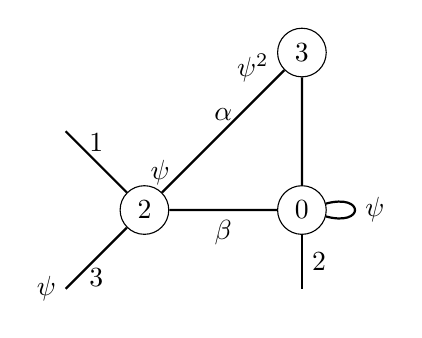
\begin{tikzpicture}[scale=1,transform shape,every loop/.style={}]
    \node[circle,draw] (A) at (0,0) {$2$};
    \node[circle,draw] (B) at (2,2) {$3$};
    \node[circle,draw] (C) at (2,0) {$0$};
    \draw[thick] (A) -- node[above]{$\alpha$} (B) -- (C) -- node[below]{$\beta$} (A);
    \draw[thick] (A) -- node[below]{$3$} (-1,-1);
    \draw[thick] (A) -- node[above]{$1$} (-1,1);
    \draw[thick] (C) -- node[right]{$2$} (2,-1);
    \draw[thick] (C) edge[loop right] node[right] {$\psi$} (C);
    \node[anchor=east] at (-1,-1) {$\psi$};
    \node[anchor=east] at (1.7,1.8) {$\psi^2$};
    \node[anchor=south] at (0.2,0.2) {$\psi$};
  \end{tikzpicture}
  \caption{$\ol{\mc{M}}_{7,3}$ 中的一个稳定图及相应的重言类。该稳定图描述了一个映射
    $\ol{\mc{M}}_{2,4} \times \ol{\mc{M}}_{3,2} \times \ol{\mc{M}}_{0,5} \to \ol{\mc{M}}_{7,3}$ 的像。}
  \label{fig:stablegraph}
\end{figure}

对 CohFT 的第一类作用是平移作用。设 $T \in V\ps{z}$。对 CohFT $\Omega$，我们定义
\[ (T\Omega)_{g,n}(\bv) \coloneqq \sum_m \frac{1}{m!} p_* \Omega_{g,n+m}(\bv, T,\ldots,T) \]
只要无穷和有意义。

\begin{exm}
    若 $\Omega^X$ 是光滑射影簇 $X$ 的 GW CohFT，且 $\tau \in H^2(X)$ 是除子类，那么无穷和有意义，我们可以定义 $X$ 的平移 GW CohFT $\Omega^{X,\tau}$。例如，若 $X$ 是五次三维簇且 $\tau = \frac{I_1}{I_0} H$，则平移到 $\tau$ 等同于镜像映射 $q \mapsto Q(q) = q e^{\frac{I_1}{I_0}}$。
\end{exm}

第二类作用是本节开头所述的矩阵 $R$ 的作用。设 $G_{g,n}$ 表示亏格 $g$、含 $n$ 条腿的所有稳定图的集合。那么我们定义
\[ (R\Omega)_{g,n} \coloneqq \sum_{\Gamma \in G_{g,n}} \frac{1}{\ab|\Aut \Gamma|} \on{Cont}_{\Gamma}, \]
其中 $\on{Cont}_{\Gamma}$ 由以下构造定义：
\begin{itemize}
    \item 在第 $i$ 条腿上，我们放置映射
        \[ R(-\bar{\psi}_i)^* \in \Hom(V',V) \ps{\bar{\psi}_i}; \]
    \item 在每条边上，我们放置双向量
        \[ V(\bar{\psi}_1, \bar{\psi}_2) \coloneqq \sum_{\mu} \frac{e_{\mu} \otimes e^{\mu} - R(-\bar{\psi}_1)^* e_{\mu} \otimes R(-\bar{\psi}_2)^* e^{\mu}}{\bar{\psi}_1 + \bar{\psi}_2}; \]
    \item 在每个顶点上，我们放置线性映射
        \[ \Omega_{g_v, n_v} \colon V^{\otimes n_v} \to H^*(\Mbar_{g_v, n_v}); \]
    \item 最后，我们考虑沿粘合态射 $\prod_v \Mbar_{g_v, n_v} \to \Mbar_{g,n}$ 的上同调前推。
\end{itemize}

\begin{defn}
    设 $R$ 如上。那么我们定义平移
    \[ T_R \coloneqq z (\1 - R(-z)^* \1') \in z V\ps{z}. \]
    只要有意义，我们定义
    \[ R.\Omega \coloneqq RT\Omega. \]
\end{defn}

\begin{thm}[Chang-Guo-Li {\cite[Theorem~2.7]{CGL2026}}]
    假设我们在系数 $\C\ps{q}$ 中工作。那么若
    \[ T_R \in z^2 V \ps{z} + zq V \ps{z}, \]
    $R.\Omega$ 是良定义的 CohFT。此外，若 $\dim V = \dim V'$，则 $\1'$ 是 $R.\Omega$ 的单位。
\end{thm}

关于 $R_0 \neq \mr{Id}$ 时的平移作用，我们想再作一点说明。为简单起见，我们假设 $V = V'$ 且 $R_0 \1 = c \cdot \1$ 对某常数 $c$ 成立。然后我们令 $\tilde{T}_R \coloneqq z( \1 - c R(z)^{-1} \1)$，并利用膨胀子方程计算
\begin{align*}
    T_R \Omega_{g,n}(\bv) &= \sum_{m=0}^{\infty} \frac{1}{m!} p_*\Omega_{g,n+m}(\bv, T_R, \ldots, T_R) \\
    &= \sum_{k,\ell \geq 0} \frac{1}{k!\ell!} p_* \Omega_{g,n+k+\ell}(\bv, ( (1-c^{-1})\1 \cdot \psi )^{\otimes k}, ( c^{-1} \tilde{T}_R )^{\otimes \ell}) \\
    &= \sum_{k,\ell \geq 0} \frac{(1-c^{-1})^k \cdot c^{-\ell}}{\ell!} \binom{2g-2+n+k+\ell-1}{k} p_* \Omega_{g,n+\ell}(\bv, \tilde{T}_R^{\otimes \ell}) \\
    &= \sum_{m=0}^{\infty} \frac{c^{2g-2+n}}{m!} p_* \Omega_{g,n+m}(\bv, \tilde{T}_R, \ldots, \tilde{T}_R)
\end{align*}
只要这有意义。


